\documentclass{book}
\title{\textbf{Regression}}
\author{Meow}
\date{2024-01-24}
\usepackage{amsfonts}
\usepackage{amsmath}
\usepackage{graphicx}
\usepackage{mathabx}
\DeclareMathOperator*{\argmax}{arg\,max}
\DeclareMathOperator*{\argmin}{arg\,min}
\usepackage{geometry}
\geometry{a4paper, left=2.5cm, right=2.5cm, top=2.5cm, bottom=2.5cm}

\begin{document}
\maketitle

\chapter{Supervised Learning}
A model is trained with input objects and desired output values. This model or \textit{hypothesis} maps new data to expected output values.

\section{Regression}
We have \textbf{input features} denoted as $x^i$ and we have \textbf{output features} (the target variable we're trying to predict) denoted as $y^i$. A pair $(x^i, y^i)$ is called a \textbf{training example} and the dataset is a list of $n$-training examples (\textbf{training set}). $X$ and $Y$ represent the input and output space value, respectively.

Given a training set, our \textit{learning function} $h: X \rightarrow Y$ will map an input value to an output value. This function is called the \textbf{hypothesis}.

If the target variable (output) is continuous, we have a \textit{regression} problem. If it's discrete, we have a \textit{classification} problem.

But... what makes the hypothesis useful? It's useful when it works well on \textit{new} data. But since we don't really know the kind of data we'll be working with, we need to assume that there's a relationship between the \textit{training data} and the \textit{testing data}. We assume they're drawn from the same probability distribution.

\subsection{Linear Regression}
It's a method used in supervised learning to predict a continuous value $y$ based on one or more input features $x$. The goal is to find a relationship between $x$ and $y$. We need to find the values of our coefficients such that we minimize the \textbf{error/cost/loss function}. Suppose we have a 2-input feature training set, containing living area and number of bedrooms.

Our $x$'s are vectors in $\mathbb{R}^2$, where $x_1^i$ is the i-th living area value and $x_2^i$ is the number of bedrooms of the i-th house.

We can try to use linear approximation, where we approximate $y$ as a function of $x$:
\[
h_{\theta}(x) = \theta_0 + \theta_1 x_1 + \theta_2 x_2
\]
Our $\theta_0$ is our \textit{bias} term, allowing the function to move from the origin as needed.

\begin{figure}[ht]
    \centering
    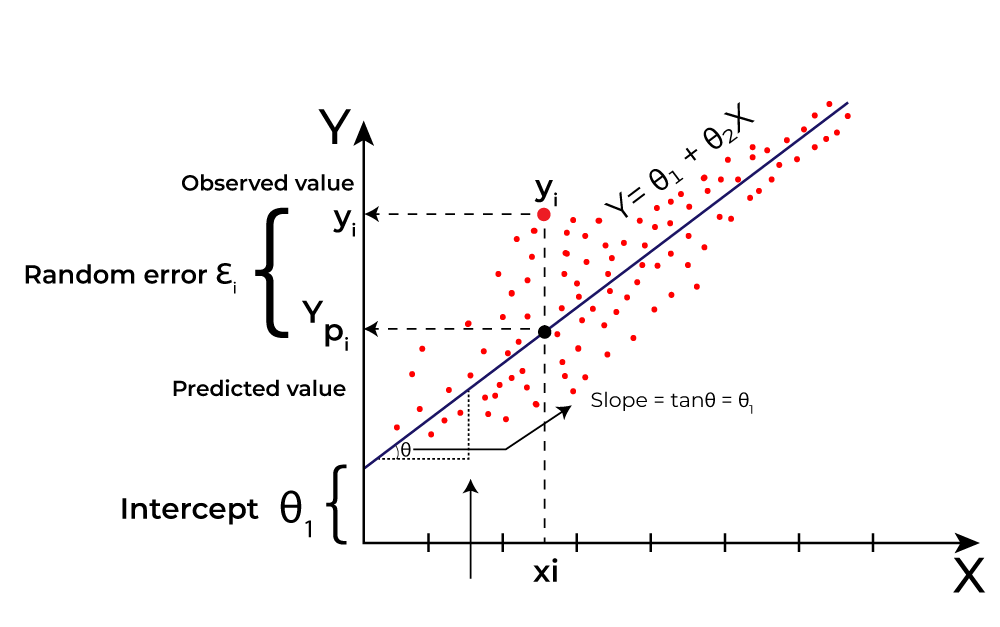
\includegraphics[width=\linewidth]{../assets/linear-reg.png}
    \caption{Linear regression example.}
\end{figure}

We can also denote it as:
\[
h(x) = \sum_{i=1}^2 \theta_i x_i = \theta^T x
\]

The accuracy of our prediction depends on \textit{irreducible} and \textit{reducible} errors. The reducible error is the error that we wish to minimize in order to make our prediction good enough. We can denote our prediction as:
\[
\hat{Y} = \hat{f}(X)
\]
where $\hat{f}$ is our estimate of $f$ and $\hat{Y}$ is our resulting prediction of $Y$.

One way of estimating the coefficients is using RSS, where we minimize the \textit{least squares} criterion. Let $\hat{y}_i = \hat{\beta}_0 + \hat{\beta}_1x_i$ be the prediction for $Y$ based on the \textit{i}th value of $X$. $e_i = y_i - \hat{y}_i$ is the \textit{i}th residual - the difference between the $\textit{i}$th observed response value and the $\textit{i}$th predicted value by the linear model. The \textbf{RSS} is defined as:
\[
\text{RSS} = e_1^2 + e_2^2 + \dots + e_n^2
\]

Least squares tries to pick the coefficient that minimizes the RSS value.

Occasionally, datasets may contain noise or irrelevant predictors which may affect our model. One way to solve that is to use a modified version of linear regression known as \textbf{ridge regression}, which minimizes the RSS and the sum of squared weights (\textbf{L2 penalty}):
\[
\text{RSS}_{\text{ridge}} = \sum_{j=1}^N (y_i - \hat{y}_j)^2 + \lambda \sum_{i=0}^D w_i^2
\]
where $\lambda \geq 0$ is a user-defined parameter that controls the weight of the penalty.

Another modified version of the linear regression idea is the \textbf{lasso regression}, which minimizes the absolute value of the weights, which we call the \textbf{L1 penalty}:
\[
\text{RSS}_{\text{lasso}} = \sum_{j=1}^N (y_i - \hat{y}_j)^2 + \lambda \sum_{i=0}^D |w_i|
\]

They both encourage our coefficients to be small, but in different ways. The two penalties are often combined to create the \textit{elastic-net penalty}:
\[
\text{RSS}_{\text{elastic}} = \sum_{j=1}^N (y_i - \hat{y}_j)^2 + \lambda \sum_{i=0}^D (\alpha w_i^2 + (1 - \alpha) |w_i|)
\]
which offers better accuracy than the two versions alone.

\subsection{How do we estimate $\hat{f}$}
We can use \textbf{parametric} methods or \textbf{non-parametric} ones. In parametric methods, we first make an assumption about the shape/form of $f$ (linear, for example) and then we try to pick a procedure that uses the training data to fit the model (ordinary least squares, for example). Be aware that there are many ways of doing these things.

$h_{\theta}(x)$ is the model's prediction of $y$ (house price) for a given house with features $x_1$ and $x_2$.

$\theta_0$ is the \textbf{intercept} or baseline price of the house when $x_1$ and $x_2$ are 0. $\theta_1$ is the weight for $x_1$. It shows how much the price increases for each square foot. $\theta_2$ represents how much the price increases for each additional bedroom.

So, we need to pick values for our $\theta$'s that are closest to our actual values in our training data. But... what does 'closest' or 'best' mean here?

The \textbf{cost function} answers that. It's a formula that measures how good our approximations to the actual value are. In linear regression, we use the \textbf{mean squared error} as the cost function:
\[
J(\theta) = \frac{1}{2} \cdot \sum_{i=1}^{n} (h_{\theta}(x^i) - y^i)^2
\]
\begin{itemize}
    \item $J_{\theta}$ is the cost function (how bad the model is at predicting)
    \item $n$: the number of training examples
    \item $y^i$: the actual value for the i-th example
    \item $(h_{\theta}(x^i) - y^i)^2$: the squared error for the i-th example.
\end{itemize}

The goal of linear regression is to find the values of $\theta$ that minimize the cost function.

\section{LMS algorithm}
It's an iterative optimization technique to adjust the parameters of our linear model, in order to minimize the \textbf{MSE} between the predicted outputs and the actual target values. Let's consider the \textbf{gradient descent} algorithm:
\[
\theta_j := \theta_j - \alpha \frac{\partial}{\partial \theta_j} J(\theta)
\]

\begin{figure}[ht]
    \centering
    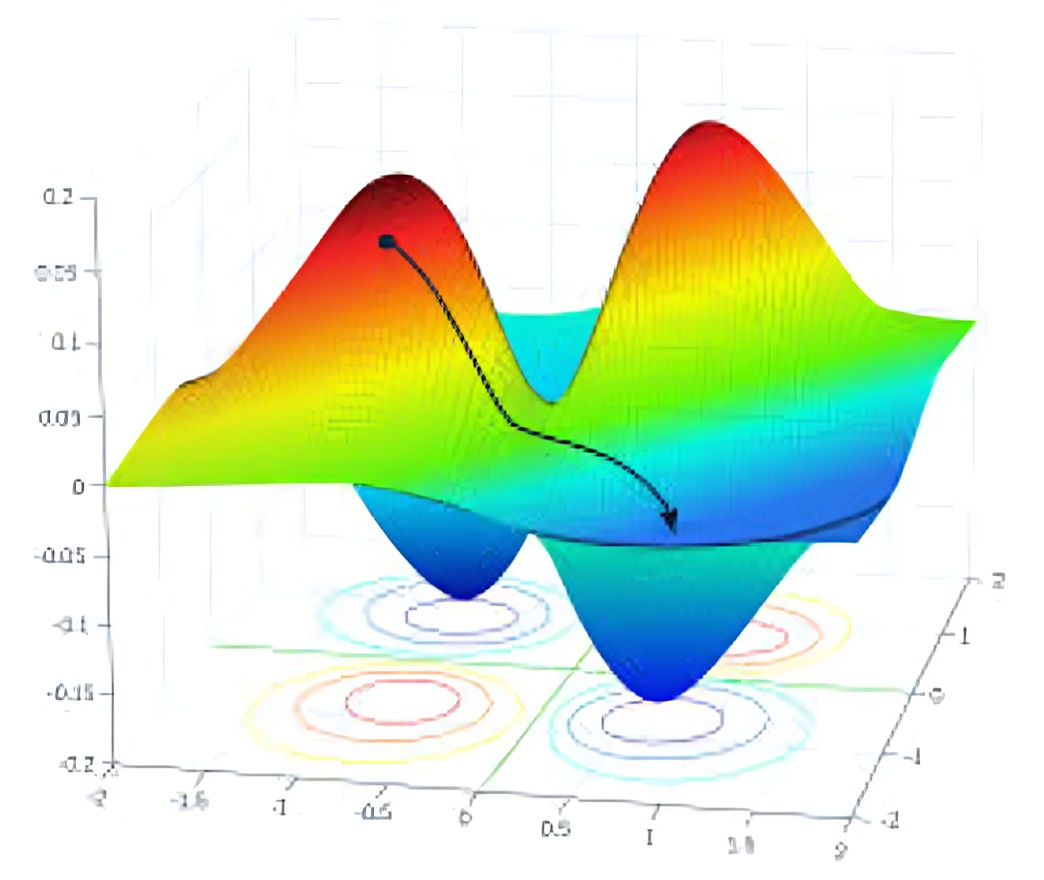
\includegraphics[width=\linewidth]{../assets/gradient-descent.png}
    \caption{Gradient descent example.}
\end{figure}

Imagine you're on a hill and you want to reach the bottom. The gradient descent is like taking baby steps according to the slope.

\begin{itemize}
    \item $\alpha$: Learning rate, it controls how big each step is.
    \item $\frac{\partial}{\partial \theta_j}$: it's the gradient of the cost function with respect to $\theta$.
\end{itemize}

We're gonna pick random $\theta$ values and adjust them until we have the best approximation possible.

Suppose we have only 1 training example:
\[
\frac{\partial}{\partial \theta_j} J(\theta) = \frac{\partial}{\partial \theta_j} \left( \frac{1}{2} (h_\theta(x) - y)^2 \right)
\]
\[
\frac{\partial}{\partial \theta_j} J(\theta) = \frac{1}{2} \cdot 2 \cdot (h_\theta(x) - y) \cdot \frac{\partial}{\partial \theta_j} (h_\theta(x) - y)
\]
\[
\frac{\partial}{\partial \theta_j} J(\theta) = (h_\theta(x) - y) \cdot \frac{\partial}{\partial \theta_j} h_\theta(x)
\]
\[
\frac{\partial}{\partial \theta_j} h_\theta(x) = x_j
\]
\[
\frac{\partial}{\partial \theta_j} J(\theta) = (h_\theta(x) - y) \cdot x_j
\]

The last line is called the \textbf{LMS update rule}. If you have more than 1 training example, you can either repeat until convergence:
\[
\frac{\partial}{\partial \theta_j} \sum_{i=1}^n (y^i - h_{\theta}(x^i)) x_j^i
\]
for every $j$.

With \textbf{batch gradient descent}, you compute the gradient over the entire training set to make an iteration:
\[
\theta_j := \theta_j + \frac{\alpha}{n} \sum_{i=1}^{n} (y^{(i)} - h_\theta(x^{(i)})) x_j^{(i)} \quad \text{for each} \, j
\]

It becomes very slow with larger datasets, obviously. Another alternative would be \textbf{stochastic gradient descent}, which runs pretty well for larger datasets. Instead of computing the gradient after scanning over the entire training set, we scan through the training set and when we find a training example, we update the parameters accordingly to best approximate the value to the actual value of it.

\subsection{Stochastic Gradient Descent (SGD)}
Stochastic Gradient Descent (SGD) is an alternative optimization method that can handle larger datasets more efficiently than batch gradient descent. Instead of computing the gradient over the entire training set, SGD computes the gradient for each individual training example. This makes it much faster, especially when the dataset is large.

In stochastic gradient descent, the update rule for the parameters $\theta_j$ after seeing a single training example $(x^i, y^i)$ becomes:
\[
\theta_j := \theta_j - \alpha \cdot (h_\theta(x^i) - y^i) \cdot x_j^i
\]
Where:
\begin{itemize}
    \item $\alpha$: Learning rate.
    \item $h_\theta(x^i)$: Model's prediction for the i-th training example.
    \item $y^i$: Actual output for the i-th training example.
    \item $x_j^i$: The value of the j-th feature of the i-th training example.
\end{itemize}

The process repeats for each training example, and we update the parameters after every example. This makes it faster than batch gradient descent for large datasets, but introduces more noise and variability in the updates. However, the noise can help the model escape local minima, leading to better overall performance.

\subsection{Mini-batch Gradient Descent}
In practice, a middle ground between batch gradient descent and stochastic gradient descent is often used, known as mini-batch gradient descent. In mini-batch gradient descent, the dataset is divided into small batches, and the gradient is computed for each batch before updating the parameters.

The update rule becomes:
\[
\theta_j := \theta_j - \alpha \cdot \frac{1}{m} \sum_{i=1}^m (h_\theta(x^{(i)}) - y^{(i)}) \cdot x_j^{(i)}
\]
Where $m$ is the size of the mini-batch. This approach combines the efficiency of stochastic gradient descent with the stability of batch gradient descent, often resulting in faster convergence.

\begin{figure}[ht]
    \centering
    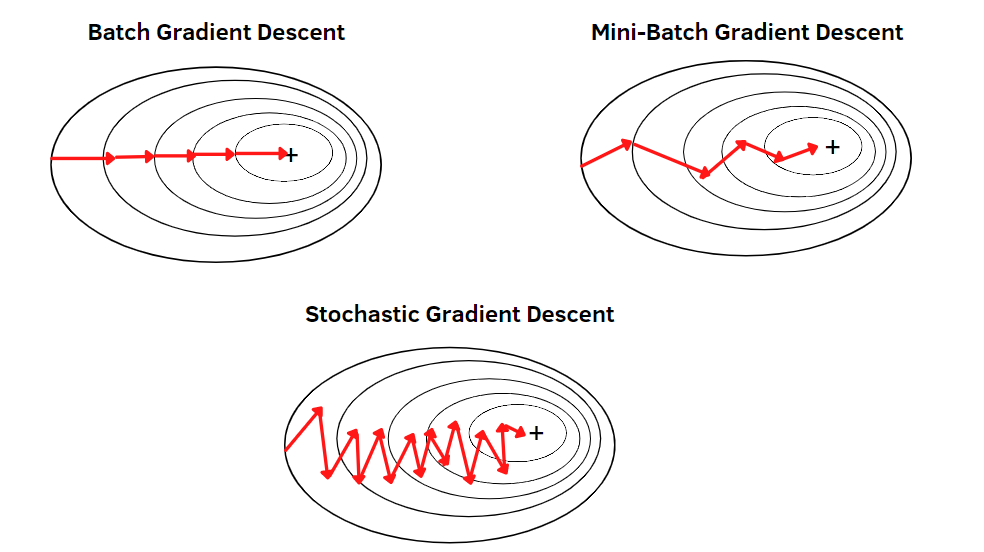
\includegraphics[width=\linewidth]{../assets/grad-descent-algorithms.png}
    \caption{Different graddient descent algorithms.}
\end{figure}

\end{document}